

% Write the full path to the location of the graphics relative to book.tex
\graphicspath{{chapters/chp1/graphics/}}

\title{Blood flow in the beating heart: Coupling fluid dynamics to reduced wall and circulation models for data-driven cardiac FSI}
\titlerunning{Blood flow in the beating heart}

\author{Marc Hirschvogel, Mia Bonini, Maximilian Balmus, David Nordsletten}
\authorrunning{Hirschvogel et al.}

\institute{Marc Hirschvogel \email{marc.hirschvogel@polimi.it} \at MOX, Dipartimento di Matematica, Politecnico di Milano, Milan, Italy}

\maketitle

\abstract{We present a fluid-reduced-solid interaction (FrSI) approach suitable for modeling blood flow in the beating left heart. 
The method uses image-derived model data to construct a suitable boundary motion space, enhanced by a reduced solid mechanics wall model to enable adaptive fluid motion. 
The method combines the efficiency of fluid dynamics models with features from full FSI approaches, uniquely integrating motion data to predict cardiac hemodynamics over a full heart cycle. 
The approach is presented for a patient-specific left heart model coupled to a lumped circulatory system, showing physiological flow behavior and pressure-volume relations.}


\section*{Introduction}
Computational fluid dynamics (CFD) provides a valuable tool to predict blood flow in the cardiovascular system \cite{schwarz2023}. 
Models of blood flow in the heart have become relevant to predict various cardiovascular conditions, where motion states from imaging are used \cite{bonini2022-suppl,zingaro2023,garciavillalba2021} or even fully-coupled fluid-solid interaction (FSI) models are employed \cite{nordsletten2011-fsi,mccormick2011modelling}. 
However, prescribed cavity motion reduces the model's ability to adapt under varying loads, and full FSI models are complex, computationally demanding, and difficult to constrain (uncertain boundary conditions and sparse patient data for reliable geometry reconstruction).
The fluid-reduced-solid interaction (FrSI) method closes the gap between model complexity and efficiency. This is a data-informed model reduction approach, particularly suited for cardiac FSI \cite{hirschvogel2024-frsi}. 
The method combines physics- with projection-based model reduction techniques that leverage Proper Orthogonal Decomposition (POD) modes derived from imaging (or some high-fidelity model) to build a reduced-order model (ROM), combined with a structural model of the ventricular wall defined on a 2D manifold.
In this contribution, we show the FrSI method's applicability to a complex, patient-specific left heart model, with a particular focus on monolithic solver implementations in FEniCSx \cite{alnaes2015fenics, baratta2023dolfinx}. This method encompasses the implementation of an Arbitrary Lagrangian-Eulerian (ALE) fluid mechanics problem subject to non-local constraints (Galerkin ROM, 3D-0D coupling to lumped circulation models). 
The solver and preconditioning aspects of this model and other fluid dynamics problems under non-local boundary conditions have been introduced in \cite{hirschvogel2025-prec}.


\section*{Methods}
The fluid-reduced-solid interaction (FrSI) problem of a 3D left heart model (atrium, ventricle, aortic outflow tract) along with the underlying data sources is depicted in Fig.~\ref{fig:heart_problem}. 
In particular, domain and motion data are retrieved from time-resolved dynamic computed tomography (CT), which are subsequently mapped to a finite element mesh in order to generate a discrete space of modes using POD \cite{rathinam2003}. 
The model is further coupled to a closed-loop systemic, pulmonary, and coronary circulation system \cite{hirschvogel2017,arthurs2016} in order to provide physiologically meaningful cardiovascular loads to the 3D model.
\begin{figure}[!htp]
\centering
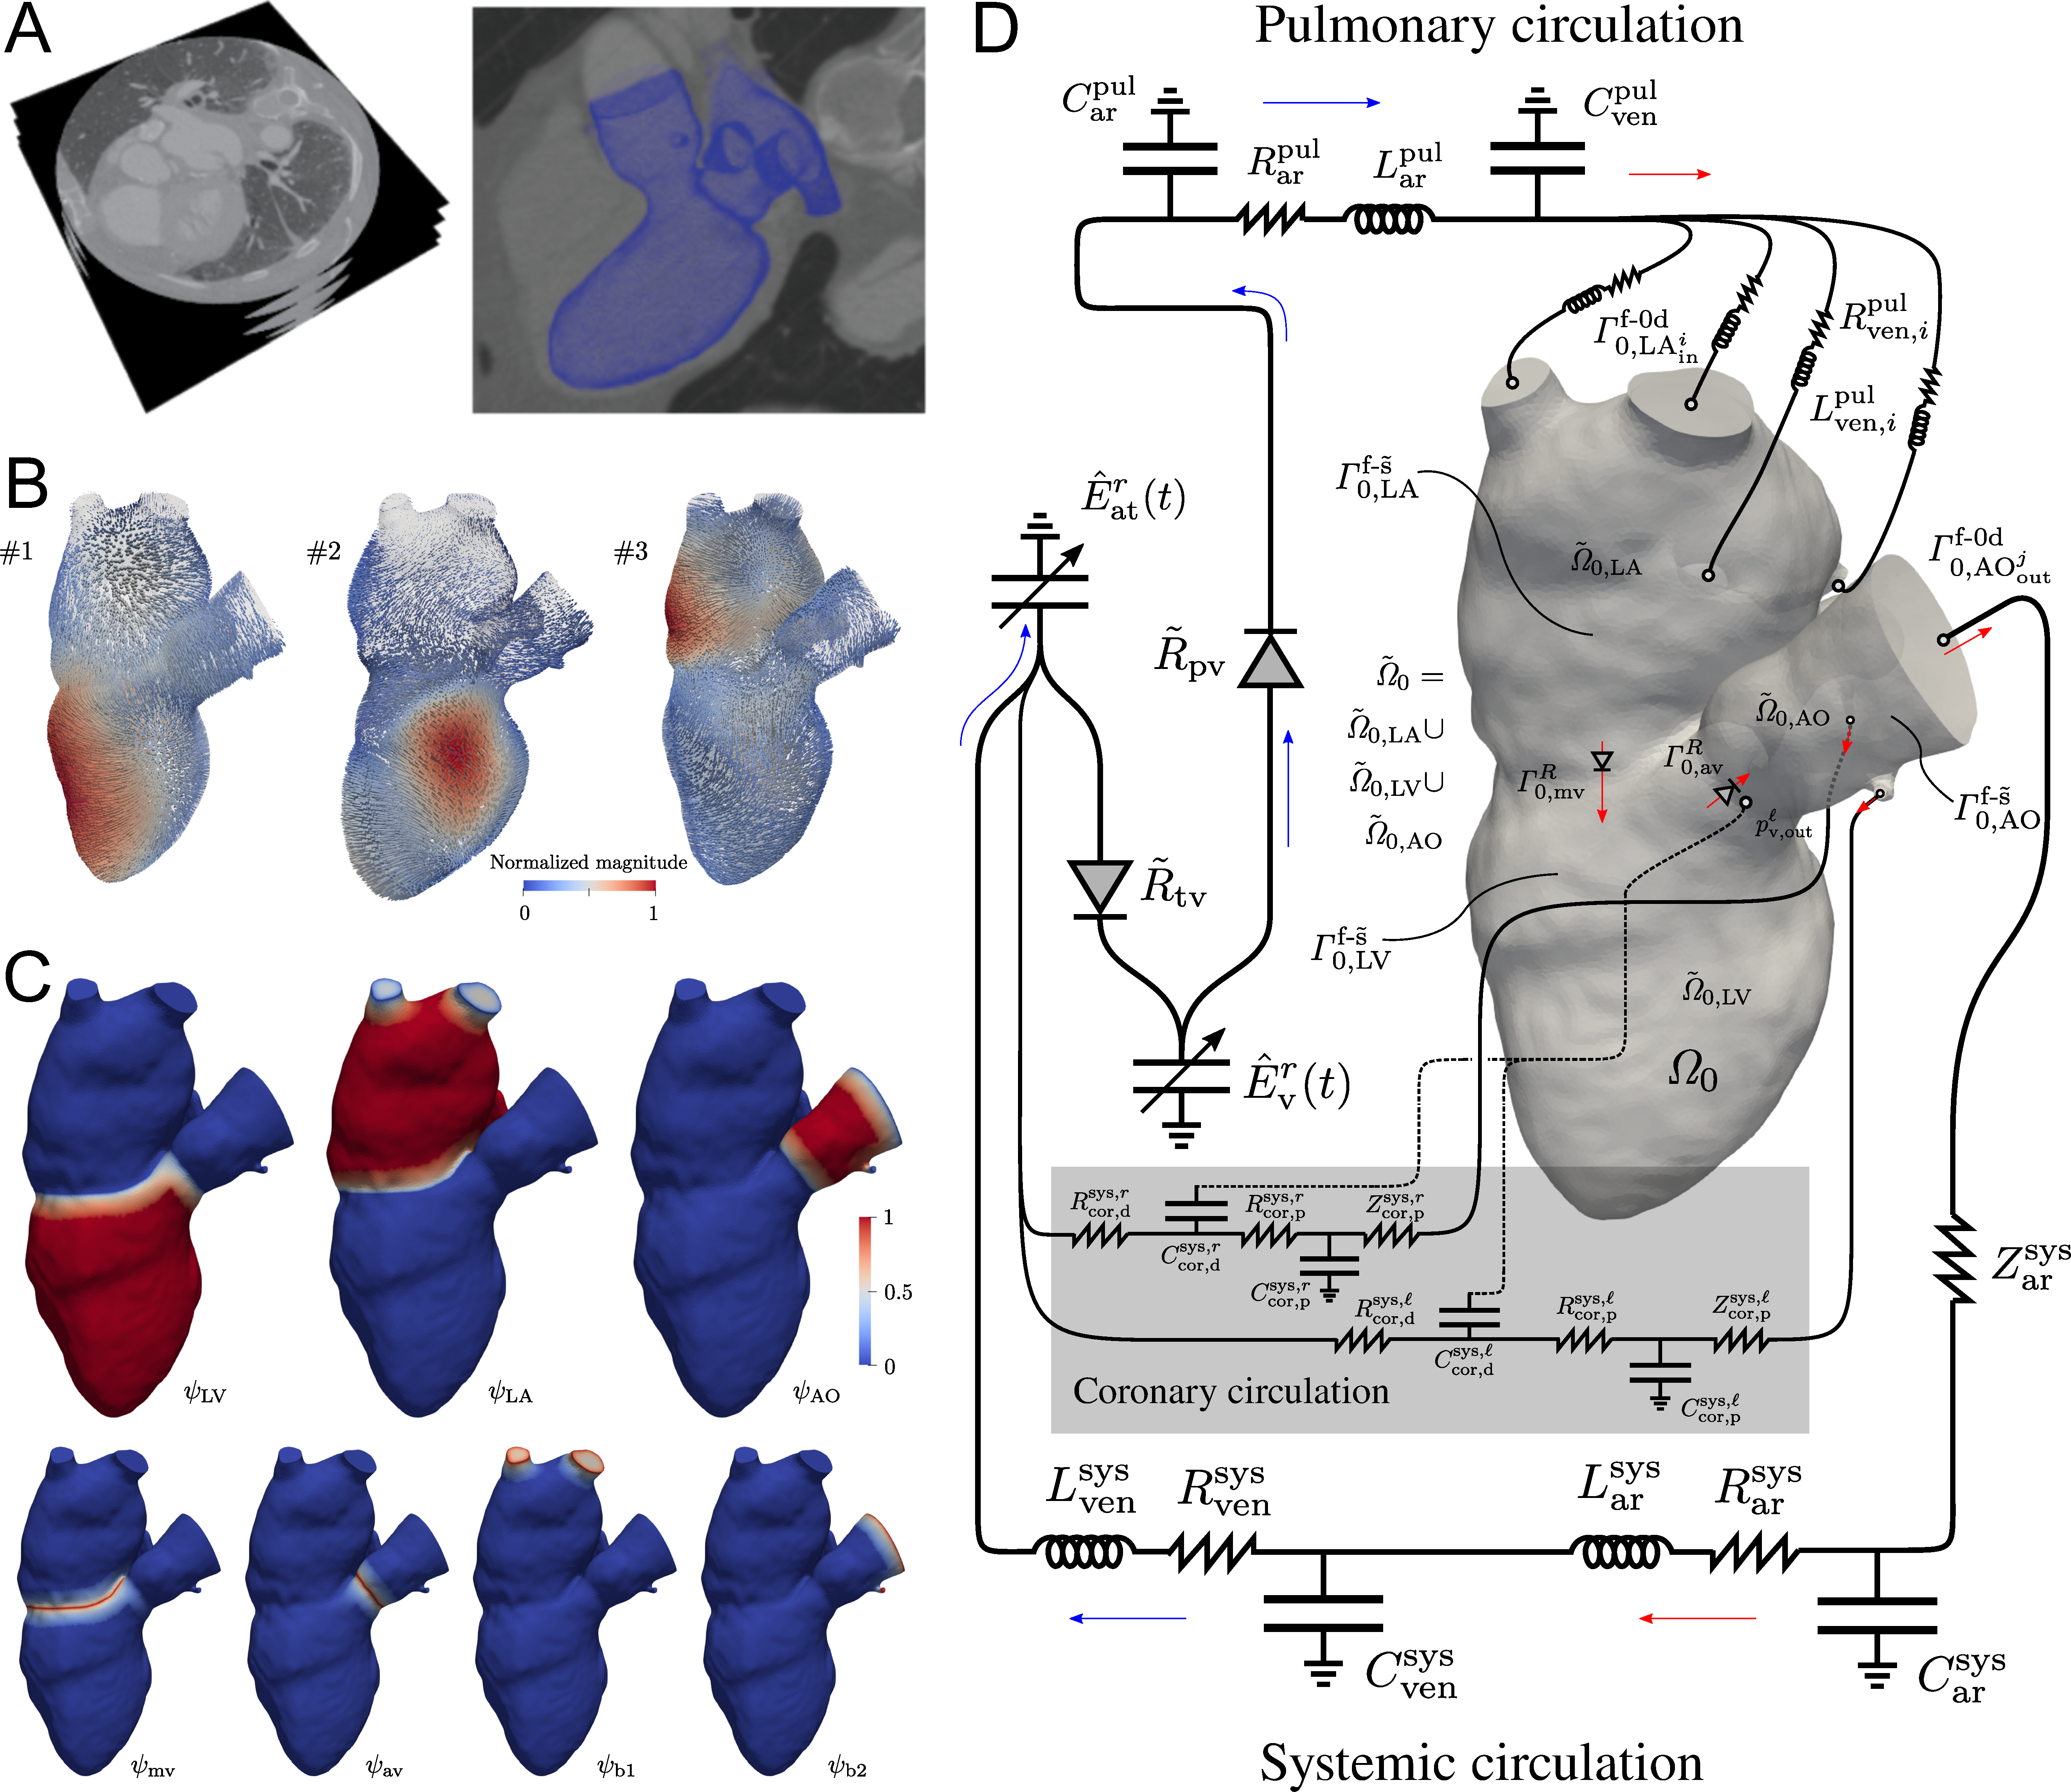
\includegraphics[width=1\textwidth]{heart_problem}
\caption{\textbf{A.} Dynamic cardiac computed tomography (CT) images with contrast and dynamic segmentation of left heart lumen for subsequent finite element mesh generation, motion tracking of deformation over the heart cycle. 
\textbf{B.} Principal component analysis by means of Proper Orthogonal Decomposition (POD) of wall motion space. The first three most dominant POD modes are shown (10 are used). 
\textbf{C.} Partition of unity fields for regional decomposition of POD space: Atrium, ventricle, and aortic outflow tract---as well as their junctions and truncations around the in-/outflows---can exhibit independent kinematics. 
\textbf{D.} 3D-0D coupled FrSI model of the left heart.}\label{fig:heart_problem}
\end{figure}

\subsection*{Preprocessing of patient data}
The FrSI approach relies on external data sourced either from some high-dimensional model or from patient-specific imaging data. Here, we build a patient-specific model of the left heart by segmenting a dynamic cardiac CT data set using 3D Slicer \cite{kikinis2014-3dslicer}, cf. Fig.~\ref{fig:heart_problem}A. Subsequently, a diastolic frame is meshed with SimModeler \cite{simmodeler}, and a motion tracking algorithm is used to extract the wall velocities at each frame and map them to the finite element mesh (with velocity degree of freedom space of size $n_{v}$). Thereafter, the wall velocity data for $m=19$ frames is collected into a snapshot matrix $\hat{\boldsymbol{\mathsf{S}}} \in \mathbb{R}^{n_{v} \times m}$, and the eigenvalue problem
\begin{align}
    (\hat{\boldsymbol{\mathsf{S}}}^{\mathrm{T}} \hat{\boldsymbol{\mathsf{S}}}) \,\boldsymbol{\uppsi}_{i} = \uplambda_{i} \,\boldsymbol{\uppsi}_{i}, \quad i = 1, \hdots, m,\label{eq:rom_eigensolve}
\end{align}
is solved, with eigenvalues $\uplambda$ and eigenvectors $\boldsymbol{\uppsi} \in \mathbb{R}^{m}$. The first $r_{v}$ POD modes $\boldsymbol{\upphi} \in \mathbb{R}^{n_{v}}$ then can be computed as follows:
\begin{align}
    \boldsymbol{\upphi}_{j} = \frac{1}{\sqrt{\uplambda_{j}}} \hat{\boldsymbol{\mathsf{S}}} \boldsymbol{\uppsi}_{j}, \quad j = 1, \hdots, r_{v}, \label{eq:phi_Phi_frsi}
\end{align}
of which the first three are shown in Fig.~\ref{fig:heart_problem}B. A suitable Galerkin model reduction operator,
\begin{align}
    \boldsymbol{\mathsf{V}}_{v}^{\mathit{\Gamma}} \in \mathbb{R}^{n_v \times (r_v + n_{v}^{\mathit{\Omega}})}, \label{eq:Vgamma}
\end{align}
then needs to be defined, with $n_{v}^{\mathit{\Omega}}$ as the size of the space of bulk (non-boundary) velocities. In Eq.~(\ref{eq:Vgamma}), POD modes Eq.~(\ref{eq:phi_Phi_frsi}) have to be incorporated such that velocity degrees of freedom on $\mathit{\Gamma}_{0}^{\mathrm{f}\text{-}\tilde{\mathrm{s}}}$ are confined to the lower-dimensional subspace, but those associated to the bulk domain remain unconstrained \cite{hirschvogel2024-frsi}. Furthermore, the POD space is decomposed with a partition of unity approach such that each region can exhibit independent kinematics, cf. Fig.~\ref{fig:heart_problem}C.

\subsection*{Strong form problem statement}
Here, we briefly state the strong problem of FrSI---fluid dynamics in an ALE reference frame \cite{donea1982,duarte2004} with a reduced structural wall model---subject to non-local flux-dependent tractions at the in- and outflows. The boundary subspace projection is then performed on the discrete system presented in a later section.\\

The incompressible non-conservative ALE Navier-Stokes equations, defining the conservation of linear momentum and mass over the domain $\mathit{\mathit{\Omega}}$ is written as:
\begin{align}
	\rho\left(\left.\frac{\partial \boldsymbol{v}}{\partial t}\right|_{\boldsymbol{x}_{0}} + \nabla\boldsymbol{v} (\boldsymbol{v}-\boldsymbol{w})\right) &= \nabla\cdot\boldsymbol{\sigma} && \;\text{in}\; \mathit{\mathit{\Omega}} \times [0,T], \label{eq:ns_strong_mom}\\
	\nabla\cdot\boldsymbol{v} &= 0 && \;\text{in}\; \mathit{\mathit{\Omega}} \times [0,T], \label{eq:ns_strong_mass}
\end{align}
where $\nabla$ is the gradient operator with respect to physical space ($\nabla\boldsymbol{v}:=\frac{\partial v_{i}}{\partial x_{j}}\boldsymbol{e}_{i}\otimes\boldsymbol{e}_{j}$) and $\left.\frac{\partial (\bullet)}{\partial t}\right|_{\boldsymbol{x}_{0}}$ the time derivative in the ALE frame. Further, $\boldsymbol{v}$ and $p$ are the fluid's velocity and pressure, $\boldsymbol{w}$ is the ALE domain velocity, and $\rho=1.025\cdot 10^{-6}\;\frac{\mathrm{kg}}{\mathrm{mm}^{3}}$ the blood density. 
The ventricular blood is assumed to be a Newtonian fluid, making the Cauchy stress $\boldsymbol{\sigma} = -p \boldsymbol{I} + \mu \left(\nabla \boldsymbol{v} + (\nabla \boldsymbol{v})^{\mathrm{T}}\right)$, with the dynamic viscosity $\mu=4\cdot 10^{-6}\;\mathrm{kPa\cdot s}$. 
The fluid's boundary wall $\mathit{\Gamma}_{0}^{\mathrm{f}\text{-}\tilde{\mathrm{s}}}$ is assumed deformable and is described by a reduced solid mechanics model governed by the balance of linear momentum of finite strain elastodynamics, which entails the physics component of the FrSI method \cite{hirschvogel2024-frsi}. 
Since the displacement field at the boundary can be entirely derived from the fluid's velocity field, kinematic compatibility and continuity of tractions are readily fulfilled by incorporating the following boundary traction, cf. comparable derivations for small strain solid wall models \cite{colciago2014}:
\begin{align}
    \boldsymbol{t}_{0}^{\mathrm{f}\text{-}\tilde{\mathrm{s}}} &= -h_0\left(\rho_{0,\mathrm{s}} \frac{\partial \boldsymbol{v}}{\partial t} - \tilde{\nabla}_{0}\cdot\tilde{\boldsymbol{P}}\right) \quad &&\text{on} \; \mathit{\Gamma}_{0}^{\mathrm{f}\text{-}\tilde{\mathrm{s}}} \times [0,T], \label{eq:frsi_tsolid_gen}
\end{align}
where $\tilde{\nabla}_{0}$ is a Nabla operator with respect to the reference frame (considering only in-plane derivatives), $h_0$ a wall thickness parameter (here $10\;\mathrm{mm}$ for ventricle, $5\;\mathrm{mm}$ for atrium, and $1\;\mathrm{mm}$ for aortic arch), $\rho_{0,\mathrm{s}}=10^{-6}\;\frac{\mathrm{kg}}{\mathrm{mm}^{3}}$ the reduced solid's density, and $\tilde{\boldsymbol{P}}=\tilde{\boldsymbol{P}}(\boldsymbol{u}_{\mathrm{f}}(\boldsymbol{v}) + \boldsymbol{u}_{\mathrm{pre}}, \boldsymbol{v})$ the first Piola-Kirchhoff stress---a general function of the fluid velocity and the fluid displacement at the boundary:
\begin{align}
    \boldsymbol{u}_{\mathrm{f}}(\boldsymbol{v}) = \int\limits_{0}^{t}\boldsymbol{v}\,\mathrm{d}\bar{t}
    \label{eq:ufluid}.
\end{align}
The first Piola-Kirchhoff stress is mapped from its material counterpart, the second Piola-Kirchhoff stress, $\tilde{\boldsymbol{P}} = (\boldsymbol{F}_{\mathrm{f}} - \boldsymbol{F}_{\mathrm{f}}\,\boldsymbol{n}_{0}\otimes\boldsymbol{n}_{0}) \tilde{\boldsymbol{S}}$, with the fluid deformation gradient $\boldsymbol{F}_{\mathrm{f}} = \boldsymbol{I} + \nabla_{0}\boldsymbol{u}_{\mathrm{f}}$, using Eq.~(\ref{eq:ufluid}). By eliminating its normal components and re-defining the out-of-plane stretch on assumptions of incompressibility, a membrane right Cauchy-Green tensor, $\tilde{\boldsymbol{C}}$, for the surface as well as its time derivative can be defined. Finally, $\boldsymbol{u}_{\mathrm{pre}}$ is a prestress displacement computed by methods described in \cite{schein2021,gee2010}. More details on the kinematics and prestress for FrSI can be found in \cite{hirschvogel2024-frsi}. The constitutive equation for the reduced solid second Piola-Kirchhoff stress is
\begin{align}
\tilde{\boldsymbol{S}} = 2\frac{\partial\mathit{\Psi}(\tilde{\boldsymbol{C}})}{\partial \tilde{\boldsymbol{C}}} + 2\frac{\partial\mathit{\Psi}_{\mathrm{v}}(\dot{\tilde{\boldsymbol{C}}})}{\partial \dot{\tilde{\boldsymbol{C}}}} + \tau_{\mathrm{a}}(t) \boldsymbol{A}_{0}, \label{eq:S_red}
\end{align}
with a structural tensor $\boldsymbol{A}_{0}=\boldsymbol{I}$ for the atrium (isotropic active stress), $\boldsymbol{A}_{0}=\tilde{\boldsymbol{M}}_{0}$ for the ventricle (active stress in directions of a reduced structural tensor \cite{hirschvogel2024-frsi}), or $\boldsymbol{A}_{0}=\boldsymbol{0}$ for the aortic arch (no active stress). The active stress $\tau_{\mathrm{a}}(t)$ follows the solution of an evolution equation, cf. \cite{hirschvogel2017}. The passive elastic model is of isotropic-exponential type\footnote{While the myocardium typically exhibits highly anisotropic passive properties \cite{holzapfel2009}, it remains inconclusive how its transmurally varying fiber, sheet, and sheet-normal architecture---governing its anisotropic stiffness---can be consistently homogenized throughout the wall and mapped to a 2D surface representation. Since our focus primarily addresses adaptive fluid motion, we prefer an isotropic 2D model whose parameters easily can be calibrated to observed (diastolic) pressure-volume data.} \cite{demiray1972}, and a typical viscous pseudo-potential is used \cite{chapelle2012}.\\

The coupling to the circulatory system is expressed via $n_{\mathrm{0d}}^{\mathrm{b}}=7$ non-local constraints, enforcing consistency between the flux over the 3D-0D boundary $\mathit{\Gamma}_{i}^{\mathrm{f}\text{-}\mathrm{0d}}$ and the flux variable $q_{i}^{\mathrm{0d}}$ from the 0D model:
\begin{align}
    \int\limits_{\mathit{\Gamma}_{i}^{\mathrm{f}\text{-}\mathrm{0d}}} (\boldsymbol{v}-\widehat{\boldsymbol{w}})\cdot\boldsymbol{n}\,\mathrm{d}A &= \alpha_{i} q_{i}^{\mathrm{0d}}(\{\mathit{\Lambda}\}_{n_{\mathrm{0d}}^{\mathrm{b}}}) \quad &&\text{in} \; [0,T]. \label{eq:3d0d_constraint}
\end{align}
Therein, $\boldsymbol{n}$ is a unit outward normal of the current frame, and scaling parameters, $\alpha_i$, account for the directionality of flow, i.e. should take the value of $-1$ if a 0D flux variable is imposed as an inflow to the fluid domain, and $1$ otherwise. The multipliers $\{\mathit{\Lambda}\}_{n_{\mathrm{0d}}^{\mathrm{b}}}$ impose normal tractions (pressure loads) on their respective in-/outflow boundaries:
\begin{align}
    \boldsymbol{t}_{i}^{\mathrm{\mathrm{f}\text{-}\mathrm{0d}}} &= -\mathit{\Lambda}_{i} \,\boldsymbol{n} \quad &&\text{on} \; \mathit{\Gamma}_{i}^{\mathrm{f}\text{-}\mathrm{0d}} \times [0,T]. \label{eq:frsi_t0d_gen}
\end{align}
The deformability of the fluid domain here is described by a pseudo-solid's displacement field $\boldsymbol{d}$ governed by 
\begin{align}
    \nabla_{0}\cdot \boldsymbol{\sigma}_{\mathrm{g}} &= \boldsymbol{0} \quad &&\text{in} \;\mathit{\Omega}_{0} \times [0,T], \label{eq:ale_strong_gen}\\
    \boldsymbol{d} &= \boldsymbol{u}_{\mathrm{f}}(\boldsymbol{v}) 
    \quad &&  
    \text{on}\; \mathit{\Gamma}_{0}^{\mathrm{f}\text{-}\tilde{\mathrm{s}}} \times [0,T], \label{eq:ale_dbc_gen}
\end{align}
subject to the essential boundary condition on $\mathit{\Gamma}_{0}^{\mathrm{f}\text{-}\tilde{\mathrm{s}}}$, requiring $\boldsymbol{d}$ to take the value of the fluid displacement Eq.~(\ref{eq:ufluid}). Here, we use a fully nonlinear ALE model of coupled Neo-Hookean type \cite{holzapfel2000}, which, on the discrete space, is scaled by the inverse of the reference cell's Jacobian determinant \cite{shamanskiy2021}. This scaling allows allocating stiffness to more anisotropic boundary elements and have the more regularly shaped bulk elements bear most of the deformation. The ALE deformation gradient and its determinant---as well as the grid/ALE convective velocity in Eq.~(\ref{eq:ns_strong_mom})---are given by
\begin{align}
    \widehat{\boldsymbol{F}}=\boldsymbol{I}+\nabla_{0}\boldsymbol{d}, \quad \widehat{J}=\det\widehat{\boldsymbol{F}}, \quad \text{and} \quad \widehat{\boldsymbol{w}}=\frac{\partial\boldsymbol{d}}{\partial t}.
    \label{eq:defgrad_ale}
\end{align}


\subsection*{Weak form and linearization}
In the following, we define the continuous weak forms of the strong problem statements suitable for a monolithic finite element implementation in FEniCSx. 
For this purpose, all integrals are formulated over the respective reference domains, and all gradient operators relate to the undeformed configuration $\mathit{\Omega}_{0}$. 
The general weak problem can be stated as follows:\\

Find fluid velocity $\boldsymbol{v}$, pressure $p$, multiplier variables $\{\mathit{\Lambda}\}_{n_{\mathrm{0d}}^{\mathrm{b}}}$, and ALE domain displacements $\boldsymbol{d}$ such that conservation of linear momentum,
\begin{equation}
\begin{aligned}
    &R_{\delta v}\left(\boldsymbol{v},p,\{\mathit{\Lambda}\}_{n_{\mathrm{0d}}^{\mathrm{b}}},\boldsymbol{d};\delta\boldsymbol{v}\right) := \int\limits_{\mathit{\Omega}_0} \widehat{J} \rho  \left(\left.\frac{\partial\boldsymbol{v}}{\partial t}\right|_{\boldsymbol{x}_{0}} + \left(\nabla_{0}\boldsymbol{v}\,\widehat{\boldsymbol{F}}^{-1}\right)\,\left(\boldsymbol{v}-\widehat{\boldsymbol{w}}\right)\right) \cdot \delta\boldsymbol{v} \,\mathrm{d}V_0 \\ &
    + \int\limits_{\mathit{\Omega}_0} \widehat{J}\,\boldsymbol{\sigma}(\boldsymbol{v},p,\boldsymbol{d}) : \nabla_{0} \delta\boldsymbol{v}\,\widehat{\boldsymbol{F}}^{-1} \,\mathrm{d}V_0 + \sum\limits_{i=1}^{n_{\mathrm{0d}}^{\mathrm{b}}} \mathit{\Lambda}_{i} \int\limits_{\mathit{\Gamma}_{0,i}^{\mathrm{f}\text{-}\mathrm{0d}}} \widehat{J}\widehat{\boldsymbol{F}}^{-\mathrm{T}}\boldsymbol{n}_{0}\cdot\delta\boldsymbol{v}\,\mathrm{d}A_0 \\
    &+ \int\limits_{\mathit{\Gamma}_{0}^{\mathrm{f}\text{-}\tilde{\mathrm{s}}}} h_0 \left(\rho_{0,\mathrm{s}}\,\frac{\partial\boldsymbol{v}}{\partial t} \cdot \delta\boldsymbol{v} + \tilde{\boldsymbol{P}}\left(\boldsymbol{u}_{\mathrm{f}}(\boldsymbol{v}) + \boldsymbol{u}_{\mathrm{pre}},\boldsymbol{v}\right) : \tilde{\nabla}_{0} \delta\boldsymbol{v}\right) \,\mathrm{d}A_0 \\
    &+ R_{\delta v}^{R}(\boldsymbol{v},\boldsymbol{d};\delta\boldsymbol{v}) + S_{\delta v}^{\mathrm{D}}(\boldsymbol{v},p,\boldsymbol{d};\delta\boldsymbol{v}) + S_{\delta v}^{\mathrm{out}}(\boldsymbol{v},\boldsymbol{d};\delta\boldsymbol{v}) = 0, \label{eq:frsi_weakform_v}
\end{aligned}
\end{equation}
conservation of mass,
\begin{align}
    R_{\delta p}(\boldsymbol{v},\boldsymbol{d};\delta p) := 
    \int\limits_{\tilde{\mathit{\Omega}}_0} \widehat{J}\,\nabla_{0}\boldsymbol{v} : \widehat{\boldsymbol{F}}^{-\mathrm{T}}\delta p\,\mathrm{d}V_0 + S_{\delta p}^{\mathrm{D}}(\boldsymbol{v},p,\boldsymbol{d};\delta p) = 0,\label{eq:frsi_weakform_p}
\end{align}
constraints enforcing consistency between 0D and 3D models,
\begin{equation}
\begin{aligned}
    &R_{\delta\mathit{\Lambda}} \left(\boldsymbol{v}, \{\mathit{\Lambda}\}_{n_{\mathrm{0d}}^{\mathrm{b}}}, \boldsymbol{d}; \{\delta\mathit{\Lambda}\}_{n_{\mathrm{0d}}^{\mathrm{b}}}\right) := \\
    &\sum\limits_{i=1}^{n_{\mathrm{0d}}^{\mathrm{b}}} \left(\,\int\limits_{\mathit{\Gamma}_{0,i}^{\mathrm{f}\text{-}\mathrm{0d}}} (\boldsymbol{v}-\widehat{\boldsymbol{w}})\cdot\widehat{J}\widehat{\boldsymbol{F}}^{-\mathrm{T}}\boldsymbol{n}_{0}\,\mathrm{d}A_0 - \alpha_i\,q_{i}^{\mathrm{0d}}\left(\{\mathit{\Lambda}\}_{n_{\mathrm{0d}}^{\mathrm{b}}}\right)\right)\delta\mathit{\Lambda}_{i} = 0,
    \label{eq:frsi_3d0d_coupling_weakform}
\end{aligned}
\end{equation}
as well as ALE domain motion,
\begin{align}
    R_{\delta d}(\boldsymbol{d},\boldsymbol{v};\delta\boldsymbol{d}) &:= \int\limits_{\mathit{\Omega}_0}\boldsymbol{\sigma}_{\mathrm{g}}(\boldsymbol{d}) : \nabla_{0}\delta\boldsymbol{d}\,\mathrm{d}V_0 = 0,\label{eq:ale_weakform}
\end{align}
hold true, for all fluid velocity and pressure test functions $\left(\delta\boldsymbol{v},\, \delta p\right)$, ALE domain motion test functions ($\delta\boldsymbol{d}$), as well as multiplier test functions ($\{\delta\mathit{\Lambda}\}_{n_{\mathrm{0d}}^{\mathrm{b}}}$). The ALE problem is further subject to the essential boundary condition Eq.~(\ref{eq:ale_dbc_gen}) at the deformable interface where the reduced solid is defined. The constitutive equation for the Cauchy stress is written with respect to the reference frame, $\boldsymbol{\sigma}(\boldsymbol{v},p,\boldsymbol{d}) = -p \boldsymbol{I} + \mu \left(\nabla_0 \boldsymbol{v}\,\widehat{\boldsymbol{F}}^{-1} + \widehat{\boldsymbol{F}}^{-\mathrm{T}}(\nabla_0 \boldsymbol{v})^{\mathrm{T}}\right)$. In Eq.~(\ref{eq:frsi_weakform_v}), $R_{\delta v}^{R}(\boldsymbol{v},\boldsymbol{d};\delta\boldsymbol{v})$ is a Robin term used to impose pressure jump-dependent tractions at the mitral and aortic valve planes.
This represents a particular challenge, since effects of the mitral and aortic valves need pressure discontinuities across the interfaces of atrium and ventricle as well as ventricle and aortic root. For this purpose, very recently introduced \textit{mixed-dimensional} functionality of FEniCSx is leveraged. This allows to create sub-discretizations (of equal or lower dimension) and make use of functions defined on different but related meshes within one finite element form. Here, the function space for the fluid pressure is defined on each sub-mesh (atrium, ventricle, aorta), and hence is allowed to jump across their respective interfaces. More details on the valve models can be found in \cite{hirschvogel2025-prec}.
Furthermore, the terms $S_{\delta v}^{\mathrm{D}}(\boldsymbol{v},p,\boldsymbol{d};\delta\boldsymbol{v})$ in Eq.~(\ref{eq:frsi_weakform_v}) and $S_{\delta p}^{\mathrm{D}}(\boldsymbol{v},p,\boldsymbol{d};\delta p)$ in Eq.~(\ref{eq:frsi_weakform_p}) refer to stabilization operators suitable for first-order approximations of both fluid velocity and pressure. Here, we make use of a variant of the G2 stabilization method \cite{johnson1998,hoffman2003,hessenthaler2017}. Furthermore, to prevent backflow-induced divergence, all Neumann/3D-0D coupling boundaries are subject to an outflow stabilization \cite{esmailymoghadam2011}, referred to by the term $S_{\delta v}^{\mathrm{out}}(\boldsymbol{v},\boldsymbol{d};\delta\boldsymbol{v})$ in Eq.~(\ref{eq:frsi_weakform_v}).

Flux variables $q_{j}^{\mathrm{0d}} = \boldsymbol{\mathsf{y}}\cdot\boldsymbol{\mathsf{e}}_{j}$ in Eq.~(\ref{eq:frsi_3d0d_coupling_weakform}) are, in general, solutions to a set of $n_{\mathrm{0d}}^{\mathrm{e}}$ 0D algebraic and first-order ordinary differential equations in time, with the vector of state variables $\boldsymbol{\mathsf{y}}$ and $\boldsymbol{\mathsf{e}}_{j}$ as the $j$-th $n_{\mathrm{0d}}^{\mathrm{e}}$-dimensional unit vector. We may state the 0D problem as follows: Find 0D model variables $\boldsymbol{\mathsf{y}}$ such that
\begin{equation}
\begin{aligned}
    R_{\mathrm{0d}} \left(\boldsymbol{\mathsf{y}},\{\mathit{\Lambda}\}_{n_{\mathrm{0d}}^{\mathrm{b}}}; \delta\boldsymbol{\mathsf{y}}\right) :=
    \left(\dot{\boldsymbol{\mathsf{g}}}(\boldsymbol{\mathsf{y}},\{\mathit{\Lambda}\}_{n_{\mathrm{0d}}^{\mathrm{b}}}) + 
    \boldsymbol{\mathsf{f}}(\boldsymbol{\mathsf{y}},\{\mathit{\Lambda}\}_{n_{\mathrm{0d}}^{\mathrm{b}}})\right) \cdot \delta\boldsymbol{\mathsf{y}} = 0,
    \label{eq:0d_weakform}
\end{aligned}
\end{equation}
for all $\delta\boldsymbol{\mathsf{y}}$, where $\boldsymbol{\mathsf{g}}$ is a linear (``left-hand side'') and $\boldsymbol{\mathsf{f}}$ a possibly nonlinear (``right-hand side'') function in the variable vector $\boldsymbol{\mathsf{y}}$ and/or multipliers $\{\mathit{\Lambda}\}_{n_{\mathrm{0d}}^{\mathrm{b}}}$.\\

The linearizations of the weak forms Eq.~(\ref{eq:frsi_weakform_v})---(\ref{eq:ale_weakform}), being the derivatives in the direction of the velocity, pressure, multiplier, and domain displacement trial functions $\Delta\boldsymbol{v}$, $\Delta p$, $\{\Delta\mathit{\Lambda}\}_{n_{\mathrm{0d}}^{\mathrm{b}}}$, and $\Delta\boldsymbol{d}$, respectively, 
\begin{align}
    K_{\delta (\cdot)_{i} \Delta (\cdot)_{j}} := D_{\Delta (\bullet)_{j}} \left[R_{\delta (\cdot)_{i}}\right], \label{eq:linearizations}
\end{align}
are computed using symbolic automatic differentiation in FEniCSx, where $D_{\Delta (\bullet)_{j}}$ is the G{\^a}teaux operator with respect to the trial function $\Delta (\bullet)_{j}$. Due to the Dirichlet conditions on the ALE problem, a special consideration is needed for the derivative of the ALE residual with respect to the fluid velocity. Due to the nature of how Dirichlet conditions are applied in FEniCSx, this is taken care of post-discretization.

\subsection*{Discretization and solution}
The problem is discretized with finite elements of piecewise linear Lagrange polynomials in space and a single-step implicit finite difference scheme in time (One-step-$\theta$ scheme, with $\theta\in\;]0; 1]$).
The projection-based component of the FrSI method requires the reduced solid boundary to be projected to a lower-dimensional subspace spanned by POD modes, cf. Fig.~\ref{fig:heart_problem}B depicting the first three modes of this space. This is done by the boundary Galerkin projection operator Eq.~(\ref{eq:Vgamma}).
At the discrete assembled stage, at the current time-step indexed by $n+1$, we seek to find the discrete velocity $\boldsymbol{\mathsf{v}}_{n+1}$, pressure $\boldsymbol{\mathsf{p}}_{n+1}$, 3D-0D coupling multipliers $\boldsymbol{\mathsf{\Lambda}}_{n+1}$, and domain displacements $\boldsymbol{\mathsf{d}}_{n+1}$ satisfying
\begin{align}
    \boldsymbol{\mathsf{r}}_{n+1} = \begin{bmatrix} 
                  \boldsymbol{\mathsf{V}}_{v}^{\mathit{\Gamma}^\mathrm{T}}\boldsymbol{\mathsf{r}}_{v}(\boldsymbol{\mathsf{V}}_{v}^{\mathit{\Gamma}}\tilde{\boldsymbol{\mathsf{v}}},\boldsymbol{\mathsf{p}},\boldsymbol{\mathsf{\Lambda}},\boldsymbol{\mathsf{d}}) \\
                  \boldsymbol{\mathsf{r}}_{p}(\boldsymbol{\mathsf{p}},\boldsymbol{\mathsf{V}}_{v}^{\mathit{\Gamma}}\tilde{\boldsymbol{\mathsf{v}}},\boldsymbol{\mathsf{d}}) \\ 
                  \boldsymbol{\mathsf{r}}_{\mathit{\Lambda}} (\boldsymbol{\mathsf{\Lambda}},\boldsymbol{\mathsf{V}}_{v}^{\mathit{\Gamma}}\tilde{\boldsymbol{\mathsf{v}}},\boldsymbol{\mathsf{d}}) \\ 
                  \boldsymbol{\mathsf{r}}_{d} (\boldsymbol{\mathsf{d}},\boldsymbol{\mathsf{V}}_{v}^{\mathit{\Gamma}}\tilde{\boldsymbol{\mathsf{v}}})
               \end{bmatrix}_{n+1}
               = 
               \boldsymbol{\mathsf{0}},
               \label{eq:res_nonlin_frsi}
\end{align}
where $\boldsymbol{\mathsf{r}}_{v}$, $\boldsymbol{\mathsf{r}}_{p}$, $\boldsymbol{\mathsf{r}}_{\mathit{\Lambda}}$, and $\boldsymbol{\mathsf{r}}_{d}$ are the assembled discrete counterparts of Eq.~(\ref{eq:frsi_weakform_v})--(\ref{eq:ale_weakform}), respectively. 
The trial space projection is $\boldsymbol{\mathsf{v}} = \boldsymbol{\mathsf{V}}_{v}^{\mathit{\Gamma}} \tilde{\boldsymbol{\mathsf{v}}}$, where $\tilde{\boldsymbol{\mathsf{v}}}$ is the (partly) reduced-dimensional velocity vector.
In order to solve Eq.~(\ref{eq:res_nonlin_frsi}), a monolithic Newton scheme is employed, resulting in the linearized system of equations to solve for the variable increments in each nonlinear iteration indexed by $k+1$:
\begin{align}
    \begin{bmatrix} \boldsymbol{\mathsf{V}}_{v}^{\mathit{\Gamma}^\mathrm{T}}\boldsymbol{\mathsf{K}}_{vv}\boldsymbol{\mathsf{V}}_{v}^{\mathit{\Gamma}} & \boldsymbol{\mathsf{V}}_{v}^{\mathit{\Gamma}^\mathrm{T}}\boldsymbol{\mathsf{K}}_{vp} & \boldsymbol{\mathsf{V}}_{v}^{\mathit{\Gamma}^\mathrm{T}}\boldsymbol{\mathsf{K}}_{v\mathit{\Lambda}} & \boldsymbol{\mathsf{V}}_{v}^{\mathit{\Gamma}^\mathrm{T}}\boldsymbol{\mathsf{K}}_{vd} \\ \\ \boldsymbol{\mathsf{K}}_{pv}\boldsymbol{\mathsf{V}}_{v}^{\mathit{\Gamma}} & \boldsymbol{\mathsf{K}}_{pp} & \textcolor{lightgray}{\boldsymbol{\mathsf{0}}} & \boldsymbol{\mathsf{K}}_{pd} \\ \\  \boldsymbol{\mathsf{K}}_{\mathit{\Lambda} v}\boldsymbol{\mathsf{V}}_{v}^{\mathit{\Gamma}} & \textcolor{lightgray}{\boldsymbol{\mathsf{0}}} & \boldsymbol{\mathsf{K}}_{\mathit{\Lambda}\mathit{\Lambda}} & \boldsymbol{\mathsf{K}}_{\mathit{\Lambda} d} \\ \\ \boldsymbol{\mathsf{K}}_{dv}\boldsymbol{\mathsf{V}}_{v}^{\mathit{\Gamma}} & \textcolor{lightgray}{\boldsymbol{\mathsf{0}}} & \textcolor{lightgray}{\boldsymbol{\mathsf{0}}} & \boldsymbol{\mathsf{K}}_{dd} \end{bmatrix}_{n+1}^{k}\begin{bmatrix} \Delta\tilde{\boldsymbol{\mathsf{v}}} \\ \\ \Delta\boldsymbol{\mathsf{p}} \\ \\ \Delta\boldsymbol{\mathsf{\Lambda}} \\ \\ \Delta\boldsymbol{\mathsf{d}} \end{bmatrix}_{n+1}^{k+1}=-\begin{bmatrix} \boldsymbol{\mathsf{V}}_{v}^{\mathit{\Gamma}^\mathrm{T}}\boldsymbol{\mathsf{r}}_{v} \\ \\ \boldsymbol{\mathsf{r}}_{p} \\ \\ \boldsymbol{\mathsf{r}}_{\mathit{\Lambda}} \\ \\  \boldsymbol{\mathsf{r}}_{d} \end{bmatrix}_{n+1}^{k} \label{eq:lin_sys_rom_frsi_mono},
\end{align}
where sub-block matrices $\boldsymbol{\mathsf{K}}_{ij}$ are obtained from the assembled discrete counterparts of Eq.~(\ref{eq:linearizations}), i.e. the derivatives of the residuals in the direction of the trial functions.
Due to the lifting of Dirichlet conditions---ALE domain displacements prescribed to equal the fluid displacements on $\mathit{\Gamma}_{0}^{\mathrm{f}\text{-}\tilde{\mathrm{s}}}$, cf. Eq.~(\ref{eq:ale_dbc_gen})---special considerations have to be carried out to assemble $\boldsymbol{\mathsf{K}}_{dv}$. 
This matrix yields
\begin{align}
    \boldsymbol{\mathsf{K}}_{dv} = \gamma\left[(\boldsymbol{\mathsf{I}} - \boldsymbol{\mathsf{I}}_{f}) \boldsymbol{\mathsf{K}}_{dd} \boldsymbol{\mathsf{I}}_{f} - \boldsymbol{\mathsf{I}}_{f}\right],
\end{align}
where $\gamma$ is a time-integration factor stemming from the derivative of the fluid displacement with respect to the velocity, and $\boldsymbol{\mathsf{I}}_{f}$ is a rank-deficient identity matrix with entries only at indices relating to boundary degrees of freedom of $\mathit{\Gamma}_{0}^{\mathrm{f}\text{-}\tilde{\mathrm{s}}}$.

Within one global Newton iteration, prior to solving Eq.~(\ref{eq:lin_sys_rom_frsi_mono}), nonlinear sub-iterations (indexed by $l$) are carried out to find an equilibrium 0D flux (given the current nonlinear iterate $\boldsymbol{\mathsf{\Lambda}}_{n+1}^{k}$) solving the time-discrete version of Eq.~(\ref{eq:0d_weakform}), meaning repeated solves of the linearized 0D model system, 
\begin{equation}
\begin{aligned}
\boldsymbol{\mathsf{K}}_{n+1}^{\mathrm{0d},k,l}\Delta\boldsymbol{\mathsf{y}}_{n+1}^{k,l+1}=-\boldsymbol{\mathsf{r}}_{n+1}^{\mathrm{0d},k,l},\label{eq:lin_sys_0d}
\end{aligned}    
\end{equation}
followed by the solution of Eq.~(\ref{eq:lin_sys_rom_frsi_mono}). In Eq.~(\ref{eq:lin_sys_0d}), $\boldsymbol{\mathsf{K}}^{\mathrm{0d}}$ is computed with symbolic differentiation using SymPy \cite{meurer2017-sympy}.

\section*{Results}

Figure~\ref{fig:heart_results} shows the results of a full heart cycle simulation. The physical time of the simulation is $T=1\;\mathrm{s}$, and a time step size of $\Delta t = 0.00125\;\mathrm{s}$ was used, hence $N=800$ time steps were done. The mid-point single step time-integration method was set to Backward Euler, hence $\theta=1$. The 3D computational domain consists of $265\,722$ nodes ($1\,487\,039$ finite elements), and the overall problem size is $1\,790\,303$ degrees of freedom. The resulting linear system Eq.~(\ref{eq:lin_sys_rom_frsi_mono}) was solved with a FGMRES \cite{saad1993} algorithm, preconditioned by our recently proposed BGS-S3\texttimes 3 preconditioner \cite{hirschvogel2025-prec}. All methods are implemented in the open-source FEniCSx- \cite{baratta2023dolfinx} and PETSc-based \cite{balay2022-petsc} solver Ambit \cite{hirschvogel2024-ambit}.

\begin{figure}[!htp]
\centering
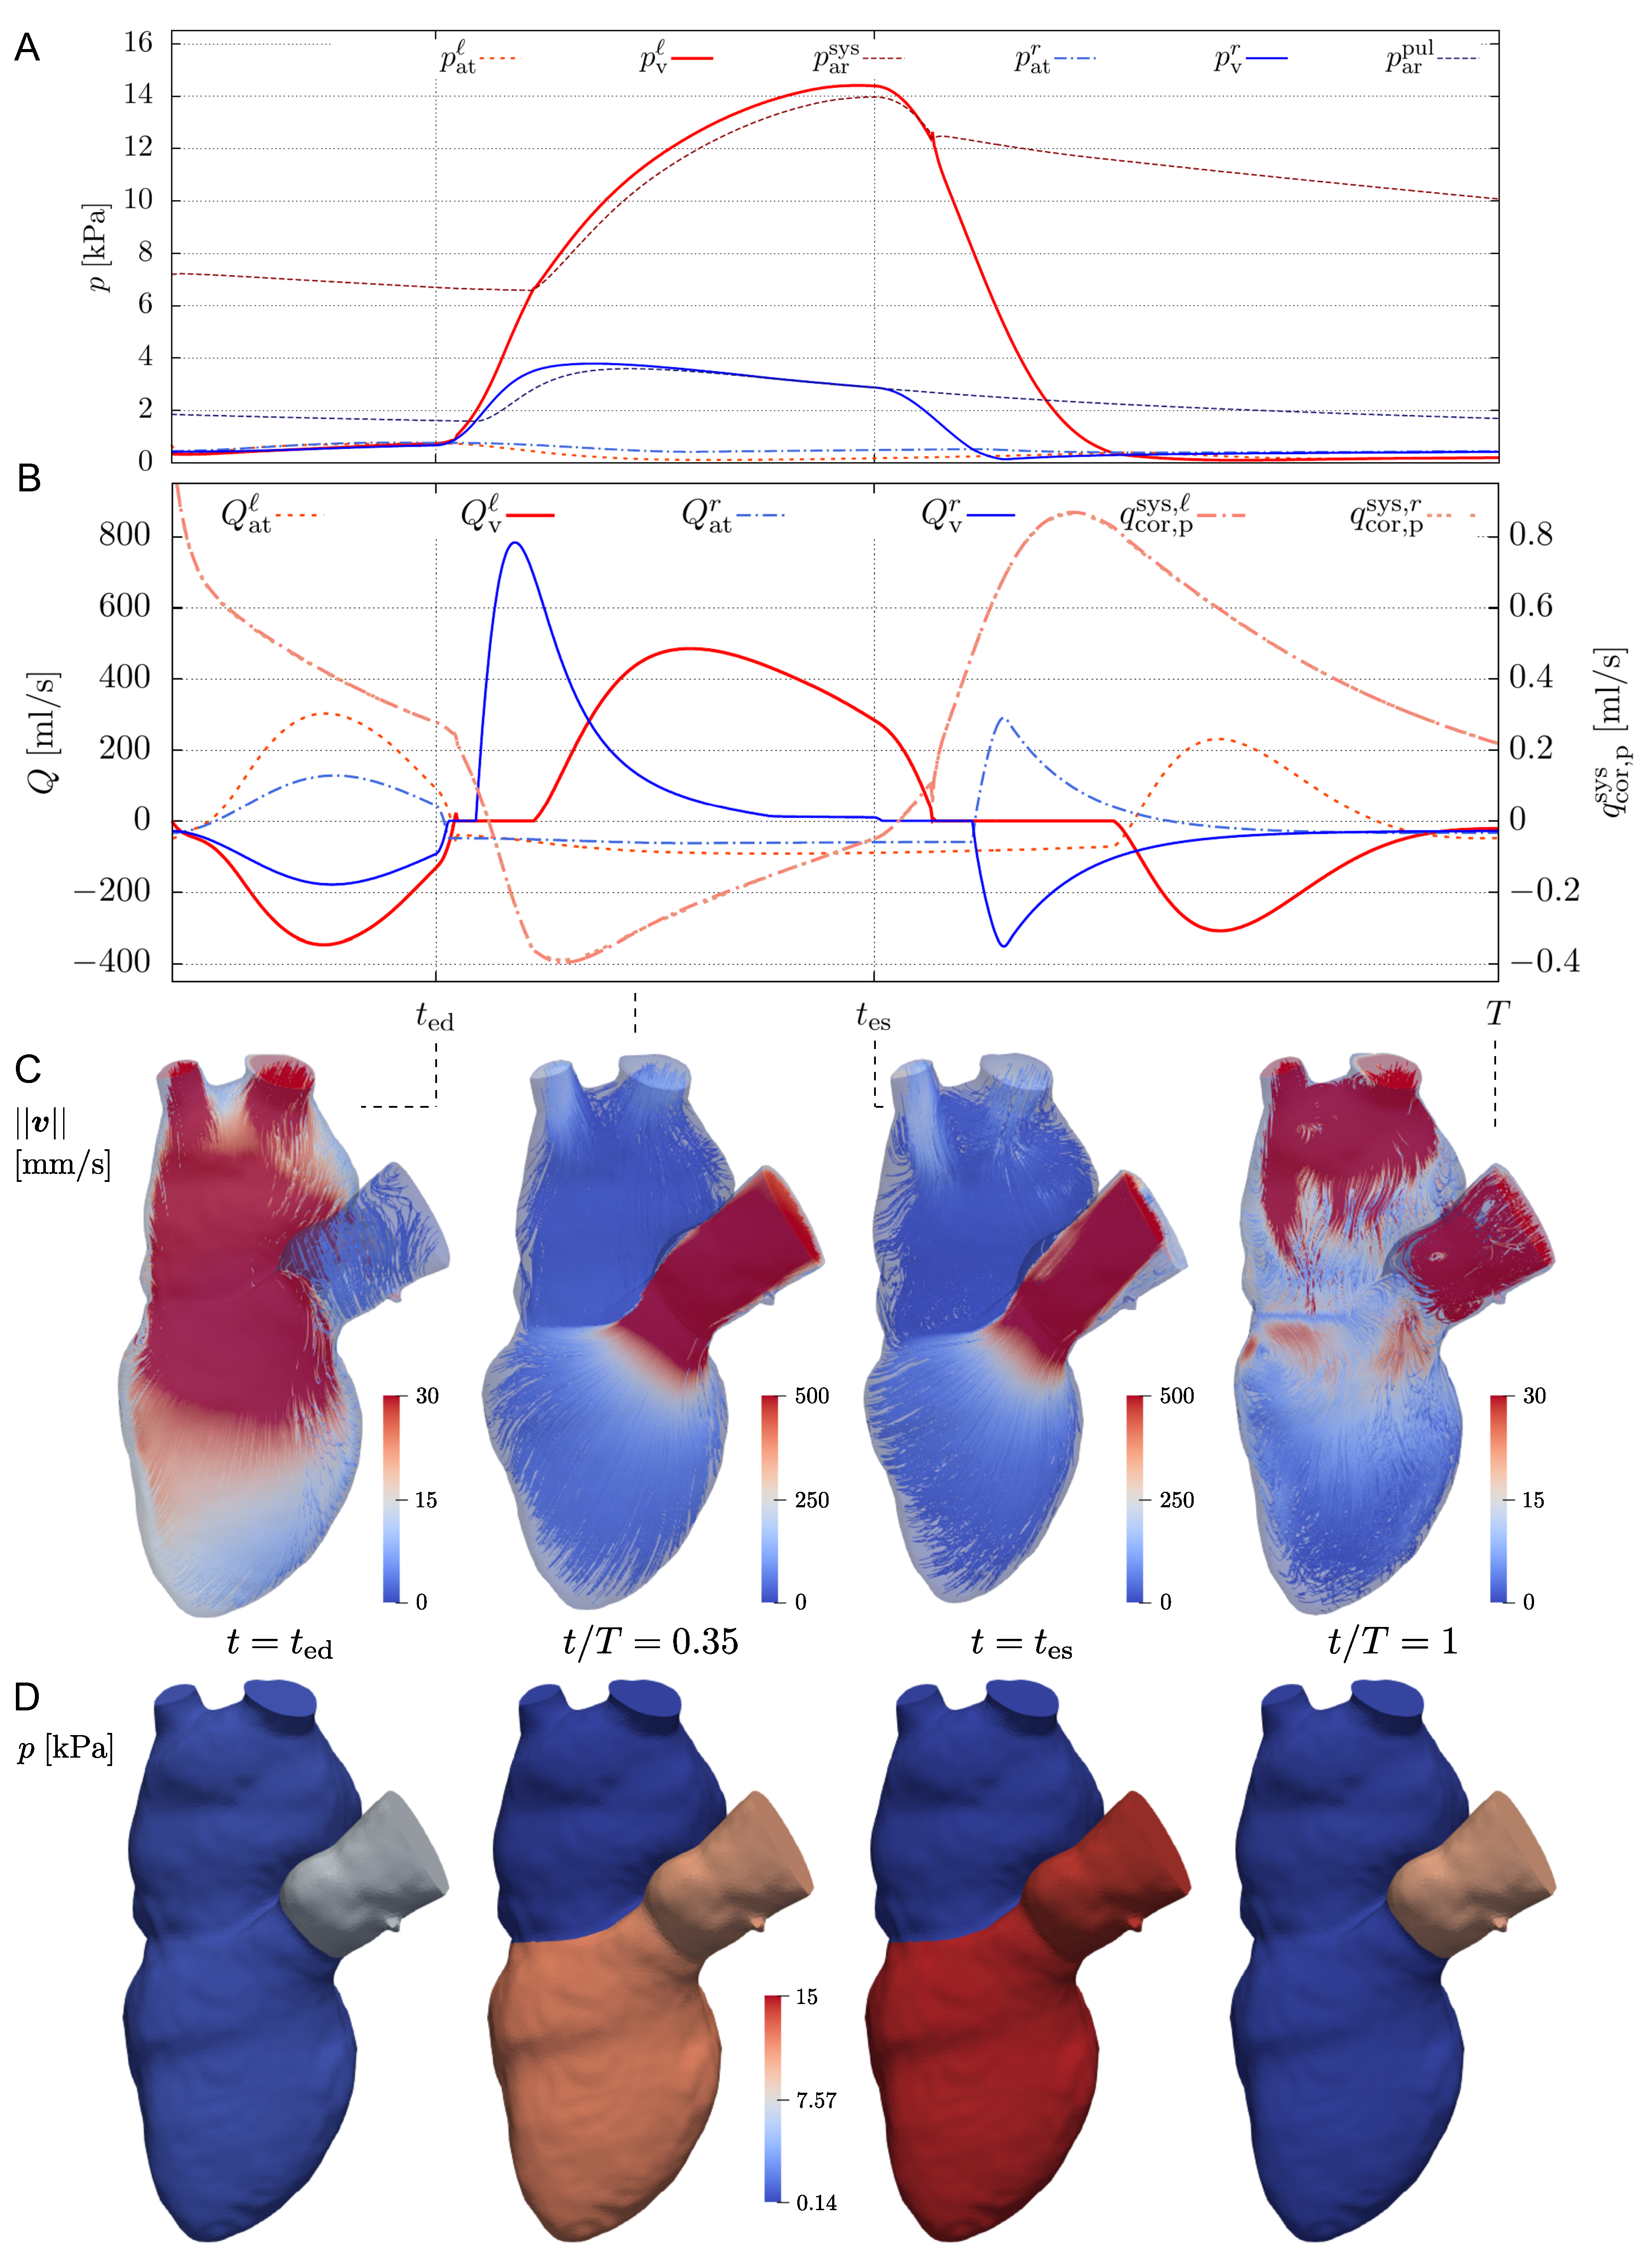
\includegraphics[width=1\textwidth]{heart_results.pdf}
\caption{Adapted from \cite{hirschvogel2025-prec}: \textbf{A.} Left atrial, left ventricular, systemic arterial, right atrial, right ventricular, and pulmonary arterial pressures over time. \textbf{B.} Left atrial, left ventricular, right atrial, right ventricular, left and right proximal coronary fluxes over time. \textbf{C.} Magnitude of fluid velocity $\boldsymbol{v}$, streamlines on longitudinal cut through deformed domain $\mathit{\Omega}$. Note the different scales for diastolic and systolic snapshots. \textbf{D.} Fluid pressure $p$, plotted on undeformed reference domain $\tilde{\mathit{\Omega}}_{0}$.}\label{fig:heart_results}
\end{figure}

\section*{Conclusion}
We presented the fluid-reduced-solid interaction (FrSI) method for a patient-specific, large-scale, left heart model, with a focus on a monolithic implementation in a FEniCSx software environment. The model can represent physiologic quantities throughout a heart cycle, and may be used to predict hemodynamics under varying cardiovascular conditions, e.g. for mitral valve regurgitation and repair.

\section*{Software and data availability}
The presented results all are computed using Ambit \cite{hirschvogel2024-ambit} release version 1.3, cf. \url{https://github.com/marchirschvogel/ambit}. All data needed to run the model---the Ambit code as well as  a medium (rf1) and fine discretization (rf2, used for generating the results presented), as well as the Ambit input file---are published at \url{https://zenodo.org/records/14631793}. Running Ambit requires FEniCSx to be installed (installation instructions at \url{https://github.com/FEniCS/dolfinx}), specifically the dolfinx development version dating to Git hash \verb\4392bc84f440d7418ec4491a4a827d50720cb7d7\ (Nov 28, 2024). The model might as well run with newer dolfinx versions, however it is not tested.

\begin{acknowledgement}
DN acknowledges funding from the Engineering and Physical Sciences Research Council Healthcare Technology Challenge Award (EP/R003866/1), and support from the Wellcome Trust EPSRC Centre of Excellence in Medical Engineering (WT 088641/Z/09/Z) and the NIHR Biomedical Research Centre at Guy's and St. Thomas' NHS Foundation Trust and KCL.    
\end{acknowledgement}

\bibliographystyle{spbasic}
% Write the full path of your bibfile relative to book.tex
\bibliography{chapters/chp1/bibliography.bib}


